\chapter{Análise do Problema}

Este capítulo tem como objetivo fazer uma análise e contextualização dos problemas descritos por esse trabalho. Na seção 3.1 é abordado sobre o conceito de evento acadêmico e seus desafios atuais. Na seção 3.2 é descrito e comparado algumas soluções presentes no mercado para gestão de eventos. Na seção 3.3 é apresentada a solução proposta por esse trabalho para auxílio na gestão de eventos da plataforma Eventos IFF. Por fim, na seção 3.4 é apresentado diagramas descrevendo o cenário do ciclo de vida dos eventos na plataforma Eventos IFF.

\section{Gestão de eventos acadêmicos}

Os eventos científicos ou acadêmicos são eventos onde ocorrem encontros entre profissionais, cientistas, especialistas e estudantes para compartilhar e obter conhecimentos sobre uma determinada área de interesse. Esses encontros promovem oportunidades para troca de experiência e atualizações sobre a área através de divulgação de novos conhecimentos \cite{lacerda}. Deste modo, os eventos acadêmicos se tornam importantes para a formação acadêmica do aluno, pois podem proporcionar diversos conhecimentos importantes para sua atuação na área.

Esses eventos podem ser compostos por diversas atividades, como: congressos, convenções, \textit{workshops}, fóruns, painéis, entre outras atividades. Além disso, em geral, os eventos acadêmicos possuem uma comissão organizadora \cite{araujo}.

Com o passar dos anos, os eventos acadêmicos passaram a ter maior visibilidade através do uso da internet, visto que antes dessa evolução, esses eventos eram apenas reconhecidos nos ambientes acadêmicos institucionalizados nas universidades \cite{araujo}. Mediante o exposto, os organizadores desses eventos passam por desafios em conseguir administrar os dados gerados antes, durante e depois do evento. Esses dados consistem, por exemplo, no registro da presença de um aluno em determinada atividade, o que é de extrema importância para a gerar o certificado de participação do aluno.

\section{Soluções no mercado}

No mercado existem algumas plataformas e aplicativos móveis que trazem soluções para gestão de eventos, cada um atendendo a critérios como: divulgação, administração de participantes, registro de presença, entre outras funcionalidades. A seguir é listada algumas das soluções mais conhecidas e utilizadas no mercado para critério de comparação e análise deste trabalho.

\subsection{Doity}

Doity é uma plataforma que oferece várias funções para gerenciamento de eventos, ou seja, desde a etapa de divulgação até a emissão de certificados. Em seu \textit{site} é informado que a Doity foi utilizada em mais 100 mil eventos presentes em mais de 1500 cidades. 

A plataforma permite realizar eventos onde a inscrição é gratuita, sem realizar nenhum tipo de cobrança pelo uso da ferramenta. A cobrança é feita quando o evento realiza inscrições pagas, onde é cobrado 10\% do valor da inscrição como taxa.

No \textit{site} da plataforma é destacada as principais soluções que a Doity proporciona. Abaixo é listado essas funcionalidades:

\begin{itemize}
    \item \textit{Site} do evento: é possível realizar a criação de uma página \textit{web} com as ferramentas da plataforma, onde o usuário consegue customizar o conteúdo, como textos, imagens e \textit{design}.
    \item Inscrições: o usuário pode realizar a inscrição no evento. Eventos onde tenha algum valor na inscrição, ele pode estar realizando o pagamento via cartão de crédito ou boleto bancário pelo \textit{site}.
    \item Credenciamento: pela plataforma é possível gerar crachás customizáveis para distribuir para os participantes. Através do crachá é possível realizar o credenciamento através do aplicativo móvel. O credenciamento envolve realizar registro de entrada e saída do participante na atividade.
    \item Inscrições em atividades: o participante pode se inscrever em cada atividade separadamente. Com isso, pela interface de gerenciamento, o organizador poderá ter um controle maior sobre as vagas nas determinadas atividades.
    \item Certificados: o organizador pode emitir certificados customizáveis pela plataforma e enviar por e-mail para os participantes, além de poder imprimir. Os certificados emitidos recebem um código de validação, que podem ser usados na plataforma da Doity para verificar a veracidade do certificado.
    \item Trabalhos científicos: a Doity oferece uma área onde o organizador pode criar um formulário customizável para envio de trabalhos científicos. Além disso, ele pode definir a forma que o trabalho poderá ser avaliado, como os critérios de avaliação e o modo de visualização das notas.
\end{itemize}

No \textit{site} da Doity contém uma área onde é possível procurar eventos cadastrados na plataforma, podendo filtrar por área, Estado, período do dia e modalidade do evento. Essa funcionalidade contribui na divulgação e procura de eventos.

Quanto à quantidade de participantes que um evento pode ter inscrito pela plataforma da Doity, para eventos onde tem valor de cobrança na inscrição, a quantidade de participantes é ilimitada. No entanto, para eventos com inscrição gratuita, existe um limite de até 3000 participantes. 

\subsection{Sympla}

A Sympla também oferece soluções para cada etapa da jornada do evento. No seu painel de controle, a plataforma conta com uma interface gráfica com várias informações em tempo real para auxiliar o organizador durante o evento, o que se torna um diferencial.

Em seu \textit{site}, a Sympla informa que foram mais de 600 mil eventos realizados utilizando a ferramenta em mais de 2500 cidades diferentes. Quanto ao custo, para eventos com inscrições gratuitas, não é cobrado algum valor, e o organizador do evento tem acesso a todas as funcionalidades da plataforma. Para eventos com valor na inscrição, a Sympla cobra 10% do valor do ingresso como taxa.

Abaixo é listado as principais funcionalidades destacadas pela Sympla:

\begin{itemize}
    \item \textit{Hotsite} para eventos: é possível criar uma simples página \textit{web} para a divulgação do evento, com ferramentas que tornam a página personalizável e responsiva.
    \item Compartilhamento de níveis de acesso: o organizador do evento pode conceder acesso para outros usuários também terem acesso ao painel administrativo da Sympla, assim dividindo a organização do evento com outros usuários. O acesso pode ser concedido com nível de acesso. Cada nível de acesso permite usar determinadas funcionalidades administrativas.
    \item Impressão de crachás para eventos: a plataforma oferece uma simples customização do conteúdo principal do crachá, podendo informar qual dado principal do participante aparecerá no crachá.
    \item \textit{Check-in}: o organizador pode realizar o credenciamento do participante por algumas formas usando a Sympla, como utilizar o aplicativo móvel para realizar a leitura de \textit{QRCode} de identificação do participante; assinalar diretamente a participação na plataforma; usar um leitor de código de barras para ler o código de barras do crachá; ou, para situações sem conexão com a internet, é possível gerar uma planilha em Excel, registrar as presenças e após isso importar no \textit{site} a planilha quando estiver com conexão com a internet novamente.
    \item Certificados de participação: é possível gerar certificados de participação e enviar para os participantes. A plataforma permite customizar o certificado.
\end{itemize}

Através do \textit{site} da Sympla é possível encontrar os eventos cadastrados na plataforma, podendo filtrar por local e categorias, por exemplo. Não foi encontrado em suas funcionalidades a possibilidade de cadastrar atividades dentro do evento, o que impossibilita registrar presença e gerar certificado por atividade, apenas de todo o evento.

\subsection{Eventbrite}

\textit{Eventbrite} oferece serviço para gerenciamento de eventos para vários países. Em seu \textit{site}, é informado que a \textit{Eventbrite} foi usada em 3 milhões de eventos em mais de 170 países durante o ano de 2017.

Em eventos com inscrição gratuita, não é cobrada taxa sobre o uso da plataforma. A \textit{Eventbrite} divide o valor de sua taxa no ingresso do evento em 3 planos, os quais estão listados abaixo:

\begin{itemize}
    \item \textit{Essentials}: taxa de 6.99\% sobre o valor do ingresso. Oferece ferramentas básicas para gerenciar o evento, como venda de ingresso \textit{online} e aplicativo móvel para organizadores.
    \item \textit{Professional}: taxa de 9,99\% sobre o valor do ingresso. Traz as mesmas ferramentas do plano \textit{Essentials}, adicionando integração com venda de ingresso em \textit{site}, formulário de compra de ingresso personalizado e análise de venda detalhada.
    \item \textit{Premium}: a taxa de cobrança deste plano tem valor customizável, passando por avaliação da \textit{Eventbrite}. Nesse plano, o usuário tem todas as mesmas ferramentas do plano \textit{Professional}, adicionando aluguel de equipamentos e treinamento para o uso da ferramenta.
\end{itemize}

No \textit{site} da \textit{Eventbrite} é destacada as principais funcionalidades que a plataforma proporciona. Abaixo é listado essas funcionalidades:

\begin{itemize}
    \item Processamento de pagamento: a plataforma permite pagamento dos ingressos do evento de forma \textit{online}, fazendo o processamento e repasse desse valor.
    \item Aplicativo para organizador: é disponibilizado um aplicativo móvel para organizadores acompanharem vários aspectos do evento em tempo real.
    \item Página de evento: é possível realizar a criação de uma página \textit{web} do evento, com \textit{design} customizável, auxiliando na divulgação.
    \item Integração com redes sociais: a \textit{Eventbrite} possui integração com redes sociais como \textit{Facebook} e \textit{Instagram}, permitindo realização de algumas ações envolvendo essas redes sociais.
    \item \textit{Check-in}: é possível realizar o credenciamento por meio de leitura de \textit{QRCode} através do aplicativo móvel do organizador.
\end{itemize}

Em relação a criação de atividades dentro de um evento, não foi encontrada funcionalidade na Eventbrite que atenda a esse critério. Quanto a geração de certificados, em seu \textit{site} é mencionada a ferramenta \textit{EB Certs} da \textit{Eventbrite} para geração de certificados customizáveis. No entanto, desde 2020 essa ferramenta se encontra inativa para uso, o que deixa sem opção para geração de certificados pela plataforma.

\subsection{Facebook Eventos}

\textit{Facebook} Eventos é uma das funcionalidades da rede social \textit{Facebook}. Essa funcionalidade não tem como foco principal auxiliar no gerenciamento de eventos, apesar de possuir ferramentas para auxiliar um pouco nesse aspecto.

O uso dessa funcionalidade traz como grande benefício o seu alcance ao público, visto que pertence a uma das maiores redes sociais atuais. Com ela, é possível definir o local e período do evento, permitindo que usuários que utilizem o \textit{Facebook}, que sejam daquela região ou tenham amigos na rede social que interagem com esse evento, recebam a divulgação desse evento.

Para ampliar a divulgação do evento, o \textit{Facebook} permite utilizar sua ferramenta de criação de anúncios para divulgação de um evento. Com ela, é possível direcionar os anúncios para o público alvo do evento. Essa funcionalidade gera um custo através de um orçamento, onde varia para o tipo de configuração feita para o anúncio e tamanho do público alvo configurado.

Além disso, como coordenador do evento criado na plataforma, é possível ver quantas pessoas selecionaram a opção que tem interesse de participar do evento, o que traz uma dimensão da adesão que o evento está tendo com o público.

Porém, como dito anteriormente, o \textit{Facebook} Eventos não tem como foco principal oferecer funcionalidades para gerenciar eventos. Com isso, não é possível registrar presença e gerar certificados através da funcionalidade.

\section{Solução proposta}

Apesar das inúmeras ofertas dispostas no mercado, foi identificado que o desenvolvimento de um aplicativo seria uma hipótese, visto os requisitos e anseios da instituição, possibilitando também demais personalizações conforme as necessidades do requisitante.

Dentre todas as supracitadas, a que mais se aproximou do desejado foi o \textit{Doity}, porém não possui integração com sistemas terceiros, possibilitando apenas um botão no site, e há limitação de participantes em eventos grátis, características as quais são essenciais.

Para a escolha da plataforma, havia como requisito características indispensáveis. A mesma deveria ser gratuita, apresentasse uma fácil integração com a plataforma Eventos IFF, emissão de certificados e possibilidade de interação entre palestrante e inscritos, sendo assim optou-se pelo desenvolvimento de uma nova ferramenta.

\section{Diagramas da solução}

Na Figura \ref{fig:caso-de-uso} é ilustrado através do diagrama de uso as funcionalidades e ações que o usuário poderá executar no aplicativo Eventos IFF. O diagrama conta com dois atores. A audiência é o usuário que tem papel de participante do evento, já o organizador é o usuário que realiza a administração do evento, tendo acesso a todas as funcionalidades administrativas do aplicativo.

\begin{figure}[H]
    \centering
    \caption{Diagrama de caso de uso}
    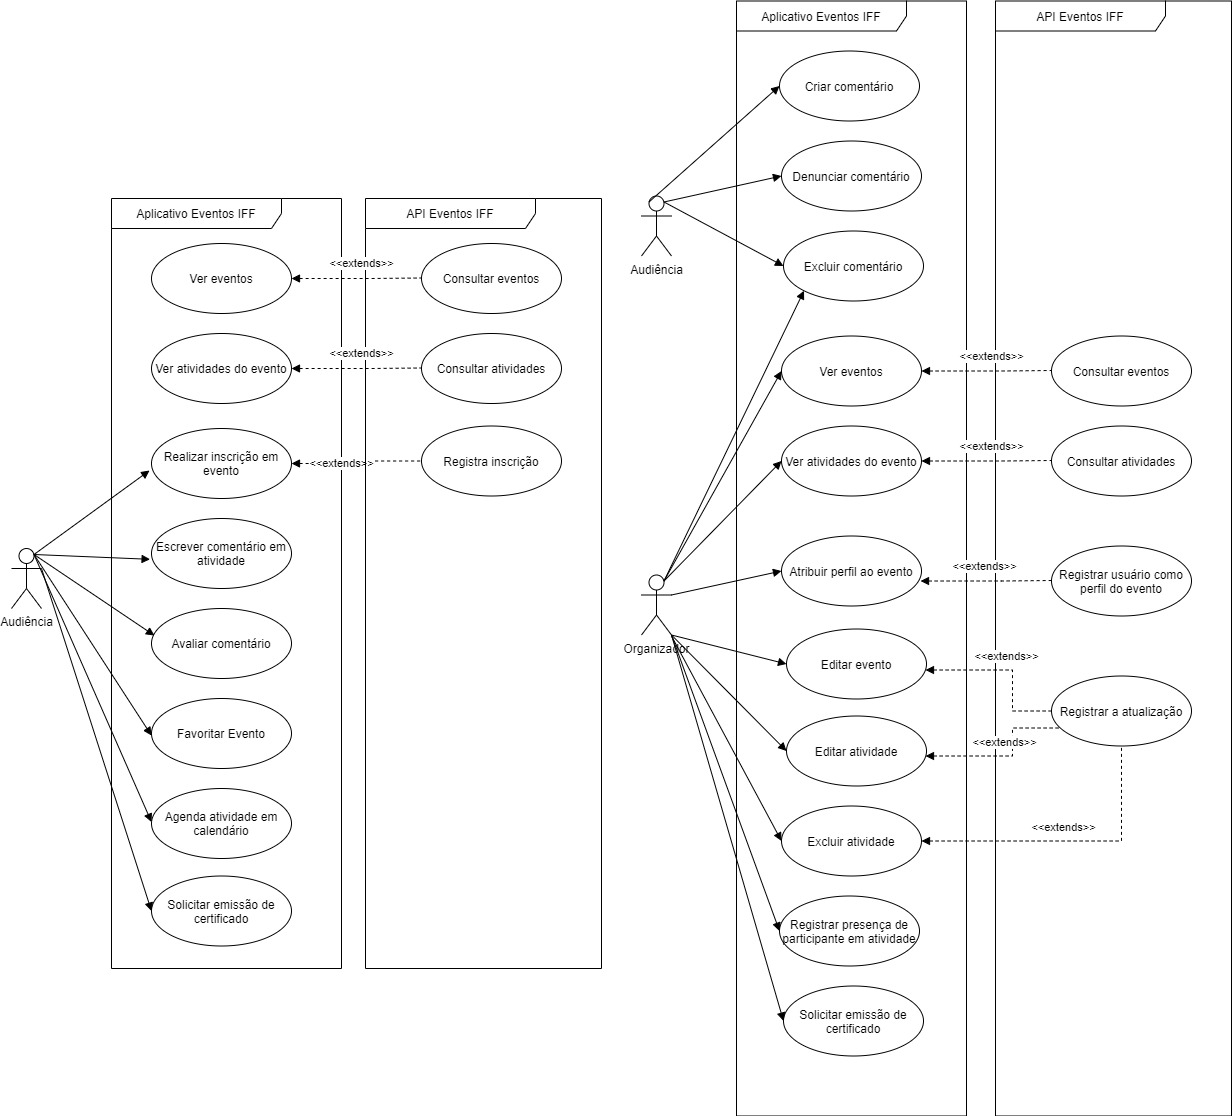
\includegraphics[scale=0.37]{figuras/caso-de-uso.jpg}
    \label{fig:caso-de-uso}
    \legend{Fonte: elaborado pelos autores}
\end{figure}

Na Figura \ref{fig:digrama-classe} é apresentado o diagrama de classe conceitual, onde é ilustrado as principais entidades que compõem o aplicativo Eventos IFF e suas relações. Também é apresentado os 4 papeis que o usuário pode ter em relação a um evento, que são: audiência, organizador, palestrante e voluntário. Cada papel possui as funcionalidades que podem executar no aplicativo.

\begin{figure}[H]
    \centering
    \caption{Diagrama de classe conceitual}
    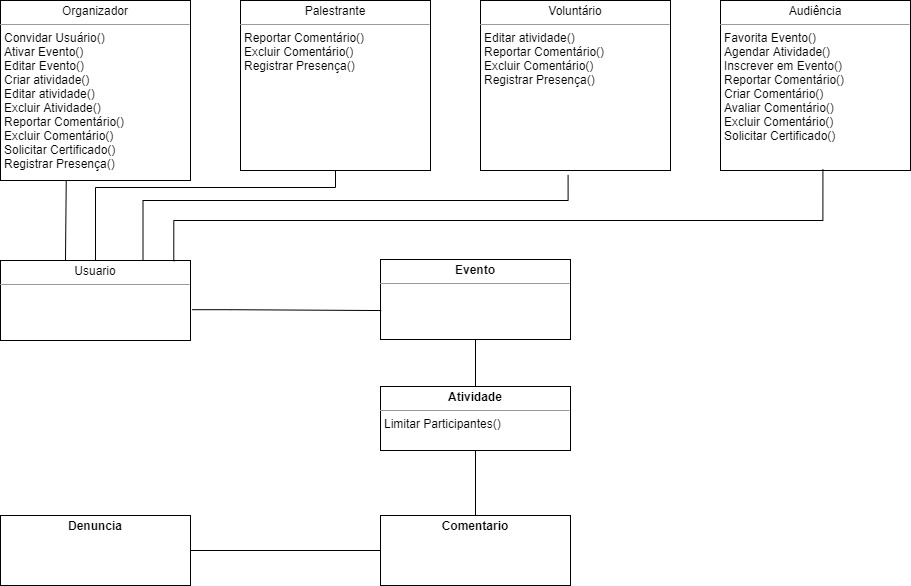
\includegraphics[scale=0.5]{figuras/diagrama-classe-conceitual.jpg}
    \label{fig:digrama-classe}
    \legend{Fonte: elaborado pelos autores}
\end{figure}